\documentclass{article}
\usepackage[T1]{fontenc}
\usepackage{lmodern}
\usepackage{graphicx}
\usepackage{amsmath,amssymb}
\usepackage[a4paper,margin=2cm]{geometry}
\usepackage[absolute,overlay]{textpos}
\setlength{\TPHorizModule}{1mm}
\setlength{\TPVertModule}{1mm}
\usepackage[indonesian]{babel}
\usepackage{hyperref}
\setlength{\emergencystretch}{2em}
% unit: Halaman 4

\begin{document}

% === Halaman 4 (llm) ===

\section*{Jenis-jenis Serangan (1)}

\vspace{133.06mm}

\begin{itemize}
    \item Berdasarkan ketersediaan informasi yang digunakan untuk menyerang sistem kriptografi:
\end{itemize}

\begin{enumerate}
    \item Chipertext-only attack
    \item Known-plaintext attack
    \item Chosen-plaintext attack
    \item Adaptive-chosen-plaintext attack
    \item Chosen-chipertext attack
\end{enumerate}

\vspace{10mm}

% deskripsi: Komik dua panel yang membandingkan imajinasi seorang 'crypto nerd' tentang menyerang sistem enkripsi RSA dengan komputer mahal versus realitas serangan fisik (pemerasan) untuk mendapatkan kata sandi.
% bbox normalisasi: [0.4770, 0.3560, 0.9330, 0.8040]
\begin{textblock*}{95.76mm}(100.17mm,105.73mm)
\noindent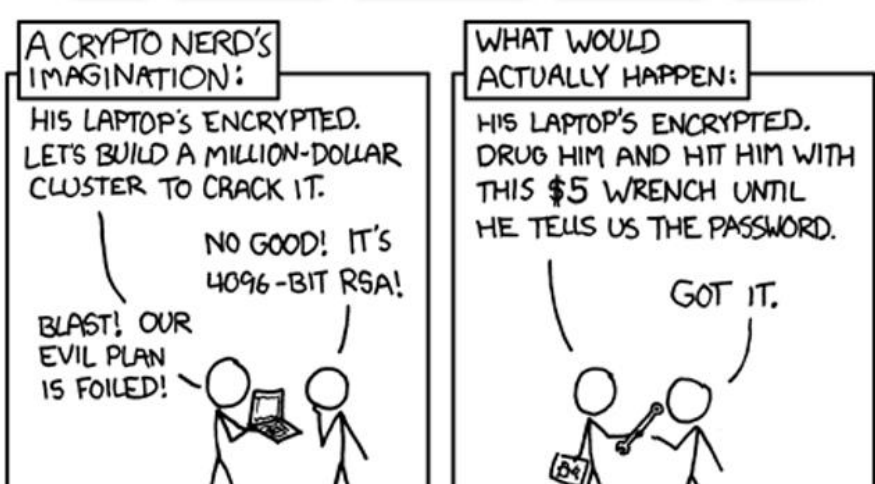
\includegraphics[width=95.76mm,height=133.06mm]{../../images/llm/page_004_img_01.png}%
\end{textblock*}

\end{document}
